Machine learning (Machine Learning) techniques have achieved remarkable performance across many domains, driven by advances in computing power and technologies \cite{alicioglu2021survey, 8022871, Chatzimparmpas_2020}. Neural networks, as a prominent Machine Learning sub-field, have demonstrated exceptional capability in identifying complex patterns within high-dimensional datasets and delivering high prediction accuracy across numerous applications \cite{alicioglu2021survey, AZODI2020442}. However, these sophisticated models present a fundamental challenge: their complex architectures makes them difficult, if not impossible, to interpret and understand directly. Neural networks are commonly referred to as "black-box" models because their internal workings and decision-making mechanisms remain opaque to human observers \cite{alicioglu2021survey}.

\subsection{Motivations for eXplainable AI}

This opacity reveals one of the most critical challenges in modern Machine Learning systems: the need for transparency and explainability \cite{alicioglu2021survey, Dağlarli20}. End-users, particularly in sensitive domains such as healthcare, transportation, defense, and finance, require a deep understanding of how classifiers generate predictions, as decision-making in these contexts often carries significant consequences \cite{alicioglu2021survey}. The ability to explain how predictions are formulated by explaining the underlying mechanisms can substantially enhance trust in Machine Learning models.

To address this need, the field of interpretable algorithms has evolved rapidly, focusing on clarifying the inner workings of black-box models \cite{alicioglu2021survey, 7536654}. A pivotal development in this area has been the emergence of \textbf{eXplainable Artificial Intelligence (XAI)} \cite{gunning2019darpa}. According to the Defense Advanced Research Projects Agency (DARPA) \cite{gunning2019darpa}, XAI is defined as "a suite of machine learning techniques that enables human users to understand, appropriately trust, and effectively manage the emerging generation of artificially intelligent partners".

% Source: DARPA's explainable artificial intelligence XAI program.pdf, Page 47
\begin{figure}[ht]
\centering
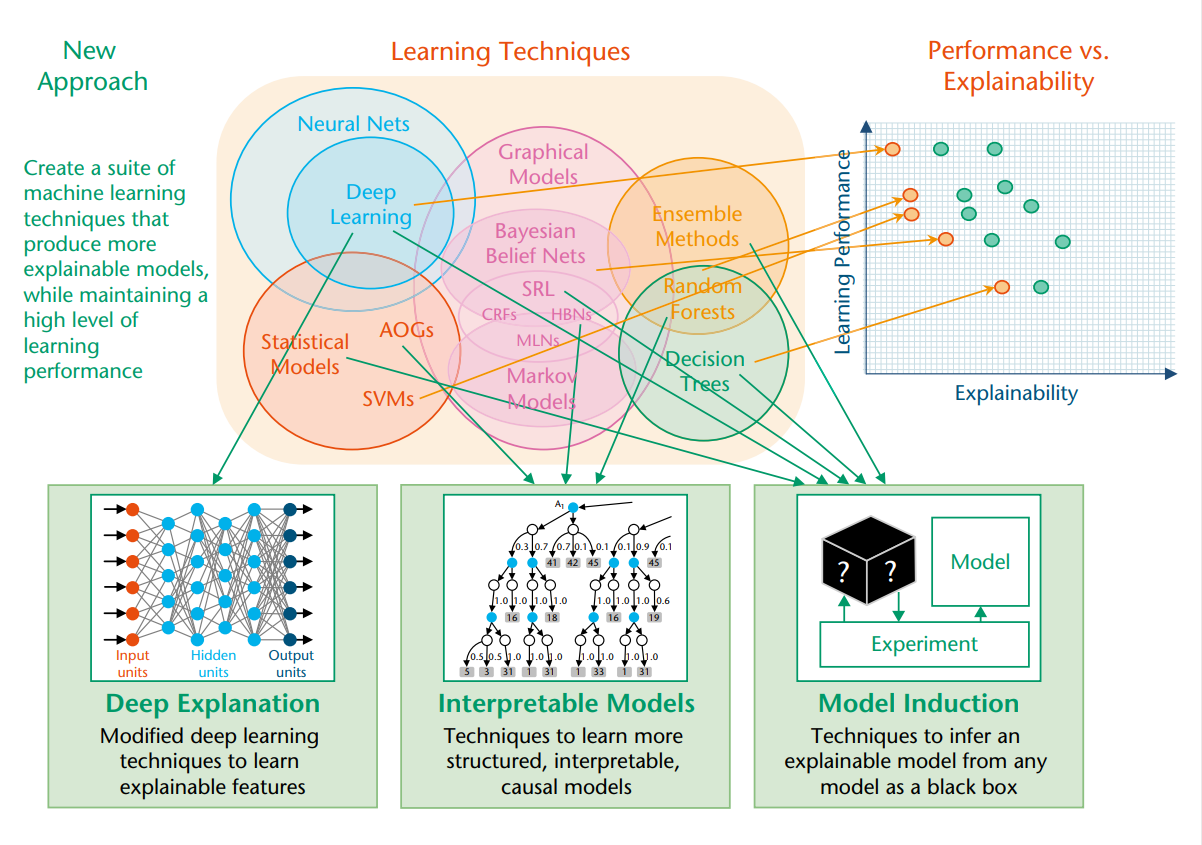
\includegraphics[width=0.8\textwidth]{images/darpa_xai_strategies.png}
\caption{Strategies for developing explainable models showing the relationship between learning techniques, performance vs explainability trade-offs, and three main XAI approaches: Deep Explanation, Interpretable Models, and Model Induction.}
\label{fig:darpa_xai_strategies}
\end{figure}

The DARPA XAI program identifies three primary strategies for developing explainable models, as illustrated in Figure \ref{fig:darpa_xai_strategies}. These approaches represent different methodological directions for addressing the fundamental trade-off between model performance and explainability.

\subsection{Defining Explainability vs. Interpretability}

While interpretability and explainability are frequently used interchangeably within the Machine Learning community, subtle yet important distinctions exist between these concepts. Biran and Cotton's \cite{Biran2017ExplanationAJ} define interpretability as "the degree to which an observer can understand the cause of a decision". From a Machine Learning perspective, interpretability encompasses understanding how decisions or predictions are generated by ML algorithms through logical reasoning. Explainability, conversely, relates more closely to the internal operational mechanisms of black-box models \cite{alicioglu2021survey}.

XAI aims to reveal the internal functioning of black-box models and the underlying reasoning of their decisions, through various methodological approaches. While domain experts inexperienced in Machine Learning typically seek understanding through reasoning and cause-effect relationships for specific decisions, Machine Learning scientists focus on the internal operational mechanisms of models, attempting to understand how individual components contribute to particular predictions \cite{alicioglu2021survey}.

\subsection{XAI Taxonomy and Approaches}

Despite the growing importance of XAI, no standardized consensus exists regarding its precise definition \cite{emmert2020explainable,adadi2018peeking,das2020opportunities}. This definitional diversity stems from varying domain-specific applications, use-case scenarios, and research objectives \cite{alicioglu2021survey}.

% Source: A survey of visual analytics for Explainable Artificial Intelligence methods.pdf, Page 4  
\begin{table}
    \centering
    \caption{Classification of the most popular XAI techniques in explaining neural networks.}
    \label{tab:xai_classification}
    \begin{adjustbox}{width=\textwidth,center}
        \begin{tabular}{|c|cc|cc|cc|}
        
        \hline
        \multirow{2}{*}{\textbf{XAI method}} & 
        \multicolumn{2}{c|}{\textbf{Explanation level}} & 
        \multicolumn{2}{c|}{\textbf{Implementation level}} & 
        \multicolumn{2}{c|}{\textbf{Model dependency}} \\
        \cline{2-7}
                                                                                     & Global     & Local      & Intrinsic  & Post hoc   & Agnostic   & Specific \\
        \hline
        ANCHORS \cite{10.5555/3504035.3504222}                                       &            & \checkmark &            & \checkmark & \checkmark &            \\
        LIME \cite{ribeiro2016should}                                                & \checkmark & \checkmark &            & \checkmark & \checkmark &            \\
        SHAP \cite{lundberg2017unified}                                              &            & \checkmark &            & \checkmark & \checkmark &            \\
        LRP \cite{Bach2015OnPE}                                                      & \checkmark & \checkmark &            & \checkmark & \checkmark &            \\
        Grad-CAM \cite{Selvaraju_2019}                                               &            & \checkmark &            & \checkmark & \checkmark &            \\
        Saliency Maps \cite{simonyan2014deepinsideconvolutionalnetworks}             &            & \checkmark &            & \checkmark & \checkmark &            \\
        Integrated Gradients \cite{sundararajan2017axiomaticattributiondeepnetworks} &            & \checkmark &            & \checkmark & \checkmark &            \\
        DeepLIFT \cite{shrikumar2019learningimportantfeaturespropagating}            &            & \checkmark &            & \checkmark & \checkmark &            \\
        Bayesian Rule Lists \cite{Letham_2015}                                       & \checkmark &            & \checkmark &            &            & \checkmark \\
        Distillation \cite{10.1145/3278721.3278725}                                  & \checkmark &            &            & \checkmark & \checkmark &            \\
        GAM \cite{10.1145/2783258.2788613}                                           & \checkmark &            & \checkmark &            &            & \checkmark \\
        Mean Decrease Impurity \cite{breiman2002manual}                              & \checkmark & \checkmark & \checkmark &            &            & \checkmark \\
        CAM \cite{7780688}                                                           &            & \checkmark &            & \checkmark & \checkmark &            \\
        \hline
        
    \end{tabular}
    \end{adjustbox}
\end{table}


XAI methods can be categorized along three primary dimensions, as shown in Table \ref{tab:xai_classification}:

\textbf{Explanation Level:} This dimension distinguishes between \textit{global explanations}, which focus on the overall model behavior and decision-making mechanisms, and \textit{local explanations}, which untangle model decisions for individual instances or subpopulations \cite{alicioglu2021survey}. Global methods such as Bayesian Rule Lists (BRL) \cite{Letham_2015}, Generalized Additive Models (GAM), and model distillation techniques provide comprehensive model-wide insights. In contrast, local methods including Local Interpretable Model-Agnostic Explanations (LIME) \cite{ribeiro2016should}, SHapley Additive exPlanations (SHAP) \cite{lundberg2017unified}, Gradient-weighted Class Activation Mapping (Grad-CAM), and Deep Learning Important FeaTures (DeepLIFT) focus on instance-specific explanations.

\textbf{Implementation Level:} This categorization distinguishes between \textit{intrinsic} and \textit{post-hoc} explanations \cite{alicioglu2021survey}. Intrinsic explanations, such as Bayesian Rule Lists and Mean Decrease Impurity (MDI), are provided directly by the model through parameters, decision trees, or rule structures. Post-hoc explanations, on the other side, analyze pre-trained models to reveal internal functioning and decision mechanisms after the training process completion.

\textbf{Model Dependency:} Methods are classified as either \textit{model-agnostic} (applicable across different model types) or \textit{model-specific} (tailored to particular architectures) \cite{bodria2023benchmarking}.

\subsection{Core Challenges and Goals}

The development of eXplainable AI is driven by interconnected objectives that address both technical and human-centered concerns. At its foundation, XAI tires to increase \textbf{trust and transparency} in AI systems by providing clear insights into their decision-making processes. This transparency is particularly crucial in high-stakes domains such as healthcare, finance, and criminal justice, where algorithmic decisions can have profound consequences on individuals' lives and where accountability is not merely desirable but legally and ethically necessary.

Beyond increasing trust, XAI must fill the gap between internal mechanisms of complex machine learning models and human comprehension. Effective explanations need to be tailored to diverse audiences, accommodating the needs of technical experts who may require algorithmic insights as well as non-specialist end-users who benefit from intuitive, accessible descriptions. This challenge of achieving multi-level interpretability represents one of the field's most persistent obstacles, as explanation systems must balance technical accuracy with cognitive accessibility.

Moreover, XAI should deliver \textbf{actionable insights} that empower users to understand not only \textit{what} decision a model has reached, but \textit{why} it arrived at that particular conclusion. This deeper level of understanding enables informed decision-making, allowing users to appropriately trust, question, or override model predictions based on contextual factors that may not be captured in the training data. Such actionability extends beyond passive understanding to active engagement with AI systems, transforming users from mere consumers of predictions into evaluators of algorithmic reasoning.

From a technical perspective, XAI techniques serve a role in \textbf{models improvement}. By revealing the internal logic of models, explanation methods facilitate debugging, bias detection, and performance enhancement, exposing potential weaknesses, unexpected behaviours, or antagonistic correlations that might otherwise remain hidden. This diagnostic capability is essential for developing robust and fair AI systems that can be safely deployed in real-world applications.

The field continues to evolve rapidly, with ongoing research addressing fundamental challenges including explanation consistency, computational efficiency, and the development of standardized evaluation metrics for explanation quality \cite{bodria2023benchmarking}. As XAI matures, the integration of visual analytics techniques with sophisticated explanation methods promises to deliver more effective human-AI collaborative systems.

\subsection{Most common XAI Algorithm}

The field of eXplainable Artificial Intelligence methods has been largely defined by two groundbreaking approaches: LIME (Local Interpretable Model-Agnostic Explanations) and SHAP (SHapley Additive exPlanations). These techniques target the same fundamental problem, how do we understand what a complex model is thinking when it makes a specific prediction? These methods represent distinct approaches to the task of instance level explainability, each proposing unique mechanisms that have influenced the development of subsequent explanation techniques.

\subsubsection{LIME: Local Interpretable Model-Agnostic Explanations}

LIME, introduced by Ribeiro et al.\cite{ribeiro2016should}, operates on the principle that complex models can be explained locally through simple, interpretable surrogate models \cite{ribeiro2016should, bodria2023benchmarking}. The core mechanism of LIME involves generating a synthetic neighborhood, around the instance to be explained, through random perturbation, where samples are drawn both in the vicinity of the target instance and further away\cite{ribeiro2016should, bodria2023benchmarking}. This neighborhood generation exploits a proximity measure $\pi_x(z)$, between an instance $z$ to the explained instance $x$, to capture locality around $x$, ensuring that nearby instances receive greater emphasis in the explanation process.

The method samples instances around the target instance $x$ by drawing nonzero elements at random, creating a perturbed dataset $\{z \in \mathbb{R}^d\}$ that is subsequently labeled by the black-box model $b(z)$ \cite{ribeiro2016should, bodria2023benchmarking}. LIME then trains a sparse linear model on these perturbed samples, with the explanation consisting of feature importance weights from this local linear approximation \cite{ribeiro2016should, guidotti2022stable}.

\textbf{Visual Affordances:} LIME's explanations are typically presented through \textit{bar charts} that display feature importance values, clearly distinguishing between positive and negative contributions to the prediction \cite{alicioglu2021survey, ribeiro2016should}. These visualizations allow end-users to easily observe both supportive and contradictory feature influences, making the local decision boundary accessible through intuitive graphical representations \cite{alicioglu2021survey}. One can observe two examples of LIME's explanations in Figure \ref{fig:LimeExpExamp}.

\begin{figure}[htbp]
    \centering
    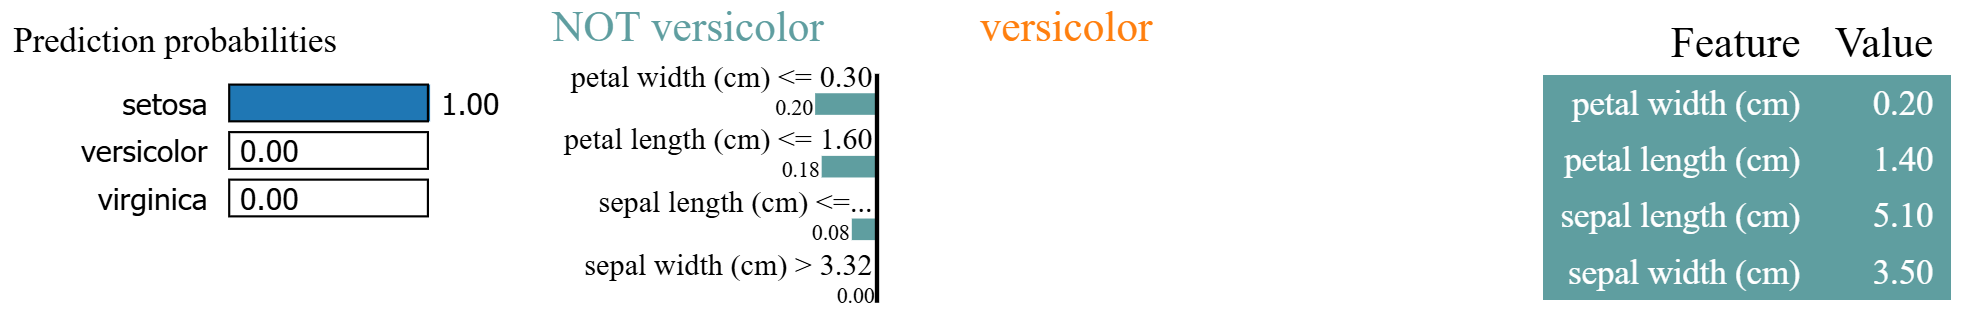
\includegraphics[width=1\textwidth]{images/limeexplain1.png}
    
    \vspace{0.5cm} 
    
    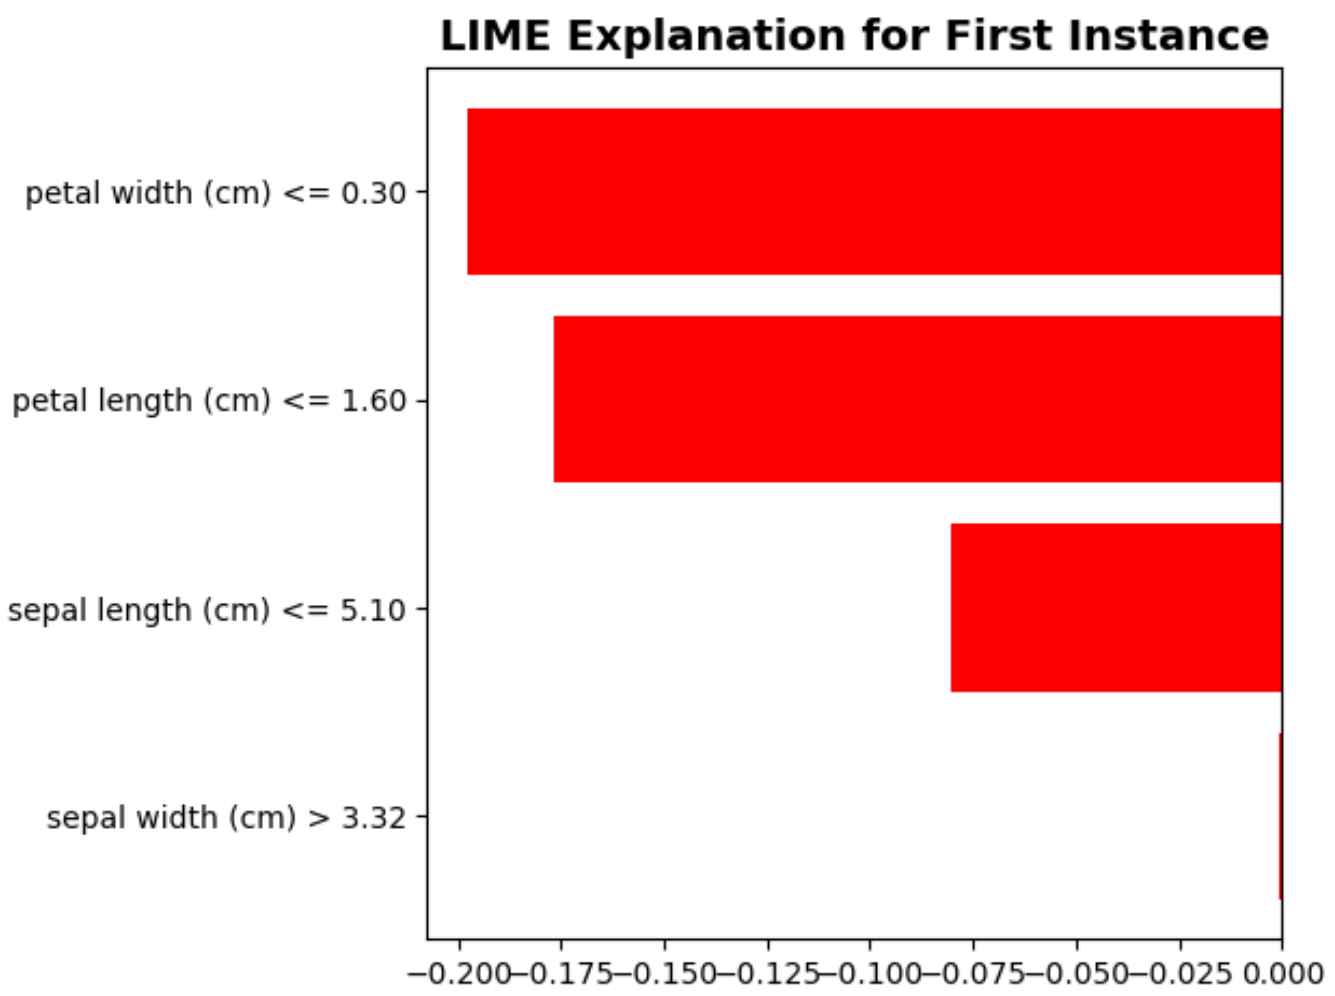
\includegraphics[width=0.6\textwidth]{images/limeexplain2.png}
    \caption{Examples of LIME explanations}
    \label{fig:LimeExpExamp}
\end{figure}

\subsubsection{SHAP: SHapley Additive exPlanations}

SHAP, developed by Lundberg et. al \cite{lundberg2017unified}, takes a fundamentally different approach rooted in cooperative game theory. The method computes feature importance through Shapley values, treating features as players in a cooperative game and calculating their marginal contributions to the prediction outcome \cite{alicioglu2021survey}. SHAP explanations are \textit{additive feature attributions} that satisfy the mathematical formulation: $g(z') = \phi_0 + \sum_{i=1}^{M} \phi_i z'_i$, where $z' \in \{0,1\}^M$, $\phi_i \in \mathbb{R}$ represent effects assigned to each feature, and $M$ denotes the number of simplified input features \cite{lundberg2017unified, bodria2023benchmarking}.

The method maintains three crucial properties: (i) \textit{local accuracy}, ensuring $f(x) = g(x') = \phi_0 + \sum^M_{i=1}\phi_ix'_i$, meaning that the explanation model $g(x')$ matches the original model $f(x)$ when $x=h_x(x')$; (ii) \textit{missingness}, where features with $x_i = 0$ have no attributed impact; and (iii) \textit{consistency}, guaranteeing that increased marginal feature contributions result in increased SHAP values \cite{lundberg2017unified, bodria2023benchmarking}. SHAP provides both local explanations for individual instances and global insights through collective SHAP value analysis \cite{bodria2023benchmarking}.

\textbf{Visual Affordances:} SHAP offers diverse visualization techniques including \textit{bar plots} that display feature importance rankings, \textit{beeswarm plots} that combine feature importance with feature effects for each sample, \textit{decision plots} showing the cumulative effect of features on individual predictions, \textit{force plots} that show how each feature pushes the prediction away from a base value, \textit{heatmap plots} for visualizing feature effects across multiple samples, \textit{image plots} designed specifically for computer vision models to highlight relevant pixels, \textit{scatter plots} that reveal the relationship between feature values and their SHAP values, \textit{text plots} for natural language processing models to highlight important words or tokens, \textit{violin summary plots} that show the distribution of SHAP values for each feature, and \textit{waterfall plots} displaying sequential feature contributions that show how each feature pushes the prediction away from a base value \cite{shapDocumentationOnline}. Some of those visualizations, on the same instance of the iris dataset as the one used in LIME's Figures \ref{fig:LimeExpExamp}, can be observed in Figure \ref{fig:shapAllViz}

\begin{figure}[htbp]
    \centering
    
    \begin{subfigure}[c]{0.385\textwidth}
        \centering
        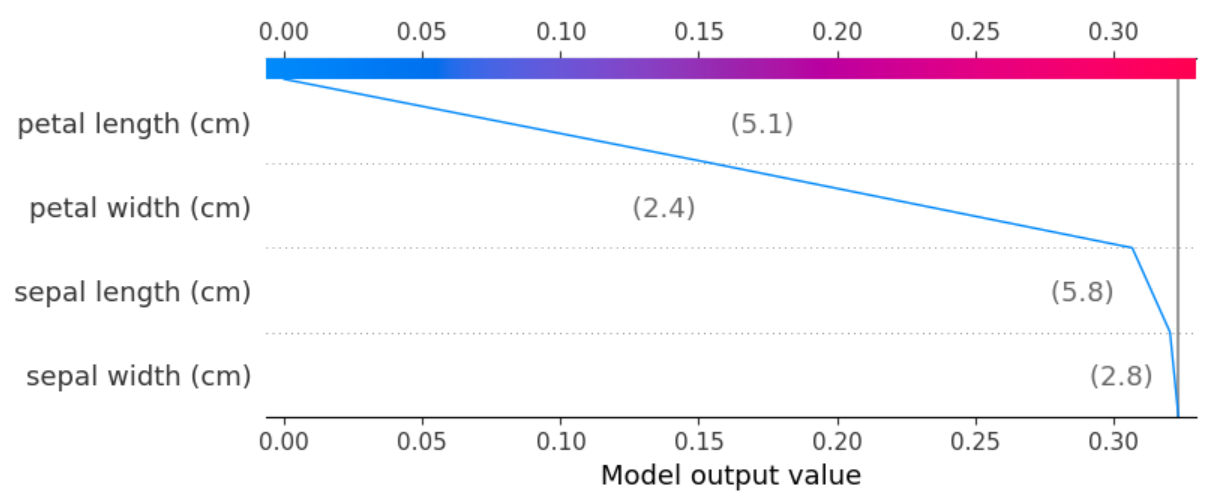
\includegraphics[width=\textwidth]{images/shapDecisionPlot.png}
        \caption{SHAP decision plot showing the cumulative impact of features on model prediction}
        \label{fig:shap_decision}
    \end{subfigure}
    \hfill
    \begin{subfigure}[c]{0.385\textwidth}
        \centering
        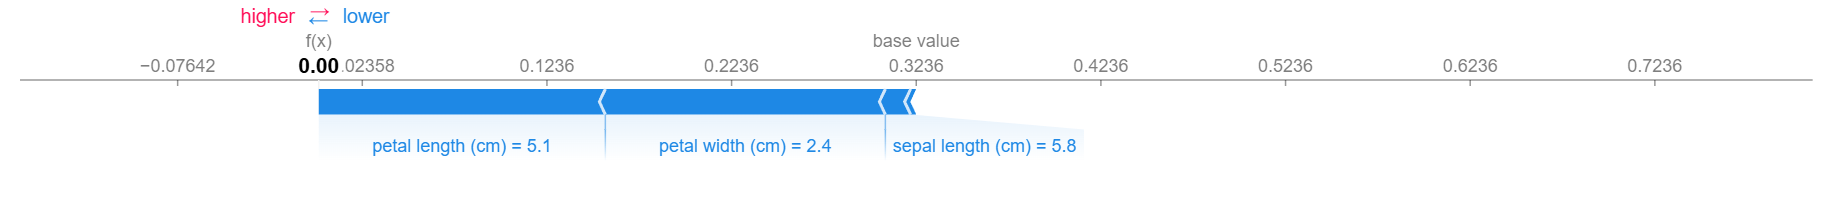
\includegraphics[width=\textwidth]{images/shapForcePlot.png}
        \caption{SHAP force plot displaying individual prediction explanation with features contributing positively (red) and negatively (blue) to push the prediction above or below the base value}
        \label{fig:shap_force}
    \end{subfigure}
    
    \vspace{0.5cm}
    
    \begin{subfigure}[c]{0.385\textwidth}
        \centering
        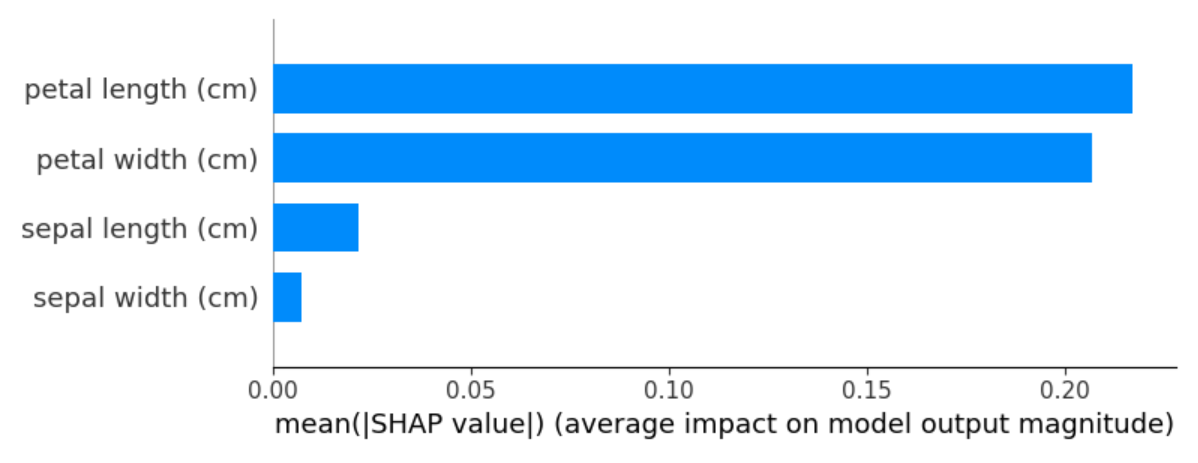
\includegraphics[width=\textwidth]{images/shapSummaryPlot.png}
        \caption{SHAP summary plot showing feature importance and impact distribution}
        \label{fig:shap_summary}
    \end{subfigure}
    \hfill
    \begin{subfigure}[c]{0.385\textwidth}
        \centering
        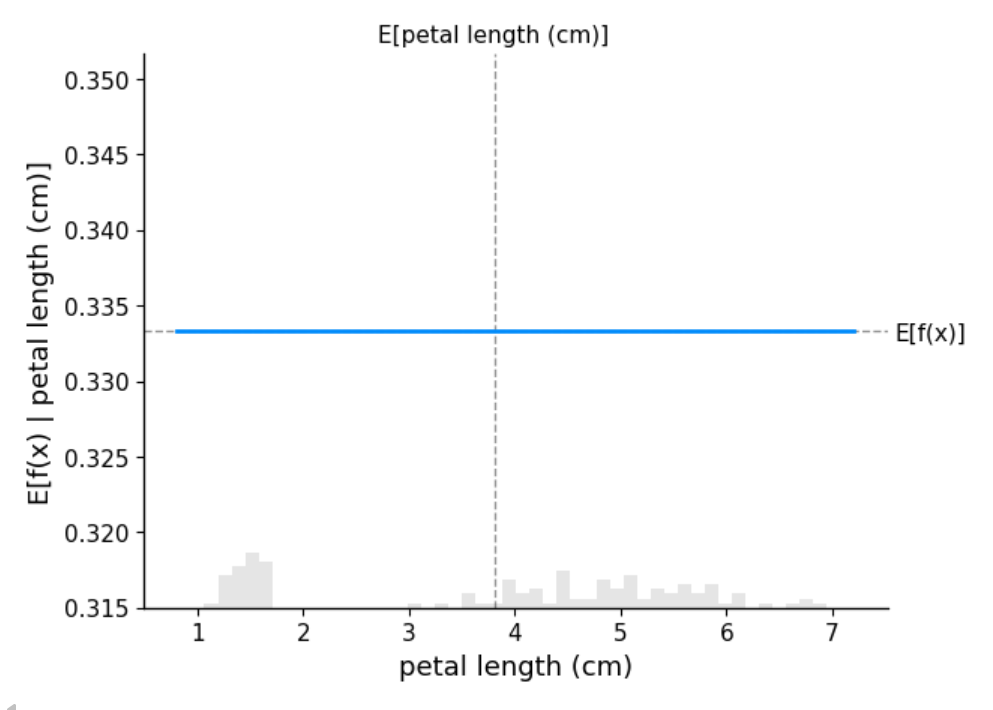
\includegraphics[width=\textwidth]{images/shapPartialDependencePlot.png}
        \caption{Partial dependence plot showing model output vs feature values}
        \label{fig:shap_dependence}
    \end{subfigure}
    
    \vspace{0.5cm}
    
    \begin{subfigure}[c]{0.385\textwidth}
        \centering
        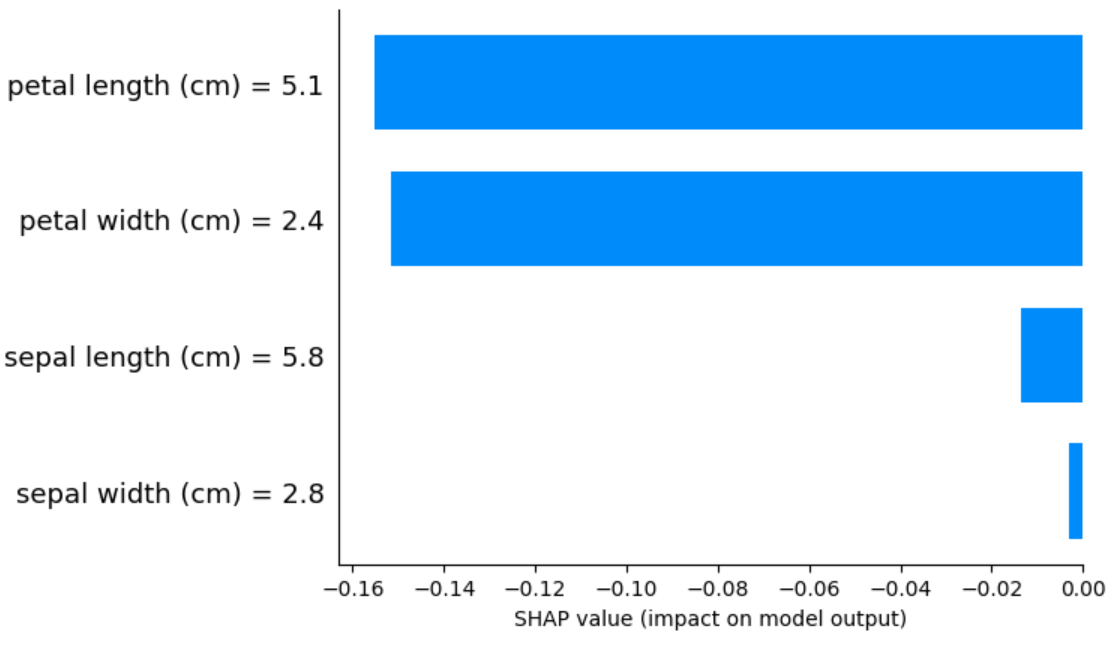
\includegraphics[width=\textwidth]{images/shapBarPlot.png}
        \caption{SHAP bar plot showing individual feature contributions}
        \label{fig:shap_bar}
    \end{subfigure}
    \hfill
    \begin{subfigure}[c]{0.385\textwidth}
        \centering
        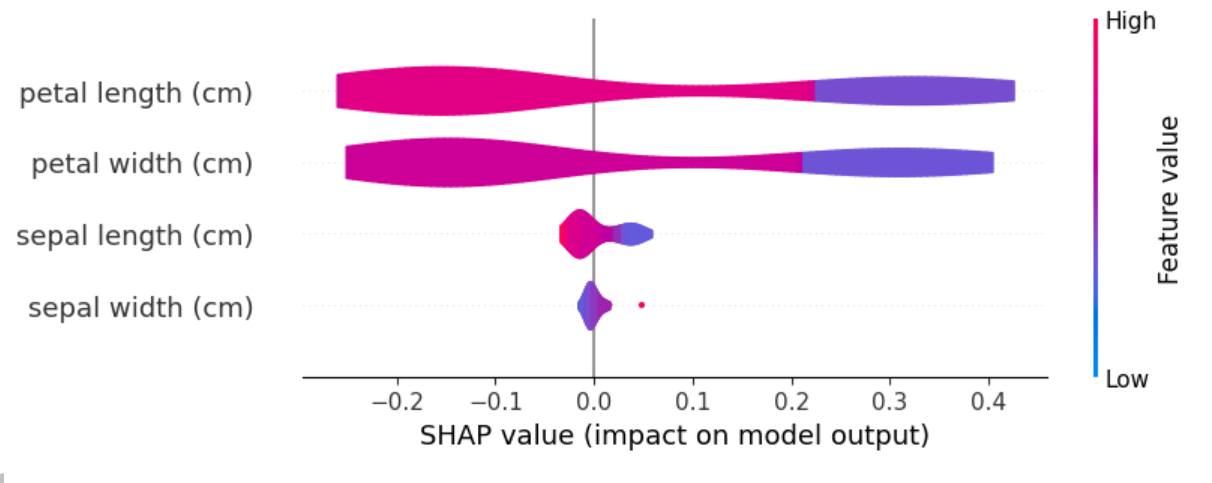
\includegraphics[width=\textwidth]{images/shapViolinPlot.png}
        \caption{SHAP violin plot showing distribution and impact of feature contributions on model predictions}
        \label{fig:shap_violin}
    \end{subfigure}
    
    \caption{Some of SHAP' visualizations showing different aspects of model interpretability on the iris dataset instance 'sepal length (cm)': 5.8, 'sepal width (cm)': 2.8, 'petal length (cm)': 5.1, 'petal width (cm)': 2.4.}
    \label{fig:shapAllViz}
\end{figure}

% Source: Opportunities and Challenges in Explainable Artificial Intelligence XAI A Survey.pdf, Page 19
\begin{figure}[ht]
\centering
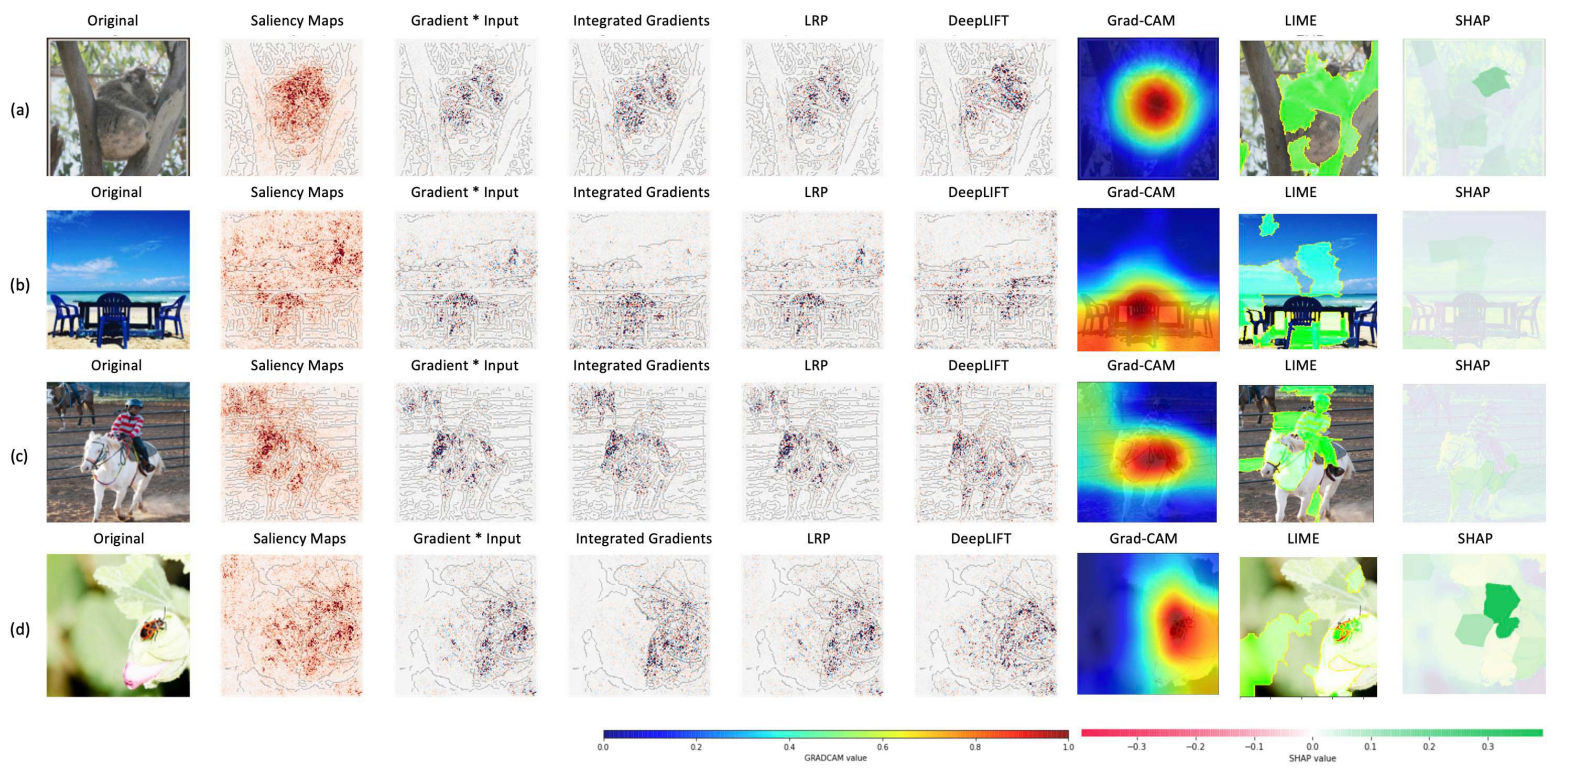
\includegraphics[width=\textwidth]{images/xai_methods_comparison.png}
\caption{Evaluation different gradient-based and perturbation-based techniques in this figure. LIME and SHAP uses segmented superpixels to understand feature importance, while gradient based saliency maps, Integrated Gradients, LRP, DeepLIFT, and Grad-CAM use backpropagation based feature importance
in a pixel level \cite{das2020opportunities}.}
\label{fig:xai_methods_comparison}
\end{figure}

\subsubsection{Comparative Analysis of LIME and SHAP}

The comparison between LIME and SHAP reveals distinct trade-offs across multiple evaluation dimensions, as demonstrated in Figure \ref{fig:xai_methods_comparison} which shows how both methods perform on real image classification tasks compared to gradient-based approaches:

\textbf{Fidelity:} As shown in Table \ref{tab:fidelity_faithfulness}, empirical evaluations demonstrate that LIME generally exhibits higher fidelity values compared to SHAP, particularly on adult dataset classifications \cite{bodria2023benchmarking}. LIME achieves fidelity scores above 90\% across most model types, while SHAP shows notably lower performance on ensemble models such as CatBoost, with values dropping to 0.777 for CatBoost on adult data and 0.670 on German credit data \cite{bodria2023benchmarking}. This suggests that LIME's linear surrogate models more accurately approximate local black-box behavior in many scenarios.

\begin{table}[ht]
    \centering
    \caption{Comparison of the fidelity and the faithfulness metrics of different explanation methods from \cite{bodria2023benchmarking}. Bold values indicate the best results. For every evaluation, the mean and the standard deviation over a subset of 50 test set records is reported}
    \label{tab:fidelity_faithfulness}
    \begin{adjustbox}{width=\textwidth,center}
    \begin{tabular}{llcccccc}
        \hline
        \textbf{Dataset} & \textbf{Black-Box} & \multicolumn{4}{c}{\textbf{Fidelity}} & \multicolumn{2}{c}{\textbf{Faithfulness}} \\
        \cline{3-6} \cline{7-8}
         &  & LIME & SHAP & ANCHOR & LORE & LIME & SHAP \\
        \hline
        adult  & LG  & 0.979 & 0.613 & \textbf{0.989} & 0.984 & 0.099 (0.30) & \textbf{0.38} (0.37) \\
               & XGB & 0.977 & 0.877 & 0.978 & \textbf{0.982} & 0.030 (0.32) & \textbf{0.36} (0.49) \\
               & CAT & 0.960 & 0.777 & 0.988 & \textbf{0.989} & 0.077 (0.32) & \textbf{0.44} (0.37) \\
        \hline
        german & LG  & \textbf{0.984} & 0.910 & 0.730 & 0.983 & \textbf{0.23 }(0.60)  & 0.19 (0.63) \\
               & XGB & \textbf{0.999} & 0.821 & 0.802 & 0.982 & 0.16 (0.26)  & \textbf{0.44 }(0.21) \\
               & CAT & 0.979 & 0.670 & 0.620 & \textbf{0.981} & 0.34 (0.33)  & \textbf{0.43 }(0.32) \\
        \hline
    \end{tabular}
    \end{adjustbox}
\end{table}

\textbf{Faithfulness:} Conversely, SHAP demonstrates superior faithfulness compared to LIME across experimental datasets \cite{bodria2023benchmarking}. For the German credit dataset, SHAP achieves faithfulness values of 0.19-0.44, while LIME scores range from 0.16-0.34. On the adult dataset, SHAP consistently outperforms LIME, achieving 0.44 faithfulness with CatBoost compared to LIME's 0.077 \cite{bodria2023benchmarking}. This indicates that SHAP explanations more accurately reflect the true feature influences despite lower fidelity scores.

\textbf{Interpretability:} Both methods offer distinct interpretability advantages. LIME's feature importance vectors are straightforward for domain experts who understand feature meanings, but may prove challenging for non-technical users when importance values are complex \cite{lundberg2017unified, bodria2023benchmarking}. SHAP's mathematical foundation provides theoretical guarantees but introduces complexity in understanding how base values, output values, and feature importance arrays combine to form explanations \cite{bodria2023benchmarking}.

\textbf{Consistency:} Both methods exhibit poor consistency performance, with neither achieving remarkable consistency according to established metrics \cite{bodria2023benchmarking}. This inconsistency represents a shared weakness across many explanation methods, highlighting the need for more robust explanation generation procedures.
